

\section*{Introduction}\label{sec:0-intro}

In Sections~\ref{sec:1-background} and~\ref{sec:2-theory}, we present the motivation for constructing simulations of high-energy proton-proton collisions, as well as the required theory for the physics behind the collision and the mathematical tools with which the process is simulated. In Section~\ref{sec:3-model} we highlight the main implementation details for the model, including the programming language of choice, UML diagrams, and essential compilation/running instructions. In Section~\ref{sec:4-results} we present results from multiple runs of our simulation model. In Section~\ref{sec:5-sensitivity-scenario} we do a sensitivity and scenario analysis to capture the solidity and stability of the model, and in Section~\ref{sec:6-verification-validation} this is elaborated on further by conducting unit tests on the various components of the model and comparing previously presented results with those from other models. Lastly, in Section~\ref{sec:7-discussion-conclusion} we briefly summarize the key findings/results from the model and highlight improvements and next steps.


\subsection*{Disclaimer}\label{sec:0-disclaimer}

It has been described via email and a number of times in previous milestones, and if it is starting to get annoying, I apologize, I just want to ensure that the unique circumstances surrounding my model are made clear and understood, because I have put a lot of work into this project, and I do not want to get points taken off simply for having a non-traditional model. This section will be almost identical to that from the previous assignment, Milestone 7, verification and validation, but with a few better explanations (I hope).

The point I want to get across about my model is that it is not similar to ordinary models like traffic models, economical models, etc. In particular, those types of models are meant to describe a wide variety of possible input/output conditions with specific ties to real-world events. For the traffic model, there are a number of input parameters to change, such as the number of cars, number of lanes in the street, speed limit, etc., and all possible variations (within reason) can relate directly to a real world possibility. Similarly, around the world and throughout time, countries' economies have varied extremely, so economical models have a high degree of freedom regarding ties to the real world.

My model, of course, is still directly tied to the real world. However, there is significantly less freedom in my choices of input parameters, scenarios, and so on, because the theory that governs proton-proton collisions (and quantum mechanics in general) is extremely tight and rigorous. One mighty popular result with which you may be familiar is the Heisenberg Uncertainty Principle, which essentially states that we cannot know both the position and the velocity of a particle at the same instant. This, and the dozens of theorems that I cannot even hope to name, highly restrict scenarios and situations which may occur in real life, and therefore limit the real-world ties present in my model.

Because of this, the latter milestones and latter sections of this project may be limited in their scope. In the context of my model, there is either: I specify particular input parameters that are accepted by the theory, and as such, get results that match what would happen in the real world, or I can specify different parameters which may break assumptions or violate the theory, in which case the results should be entirely ignored, as they not only don't represent what happens in real life, but may be simply mathematically invalid.

To reiterate, though, my model is absolutely still representative of a real world process, and as I will describe in Section~\ref{sec:1-background}, there are strong and relevent motivations for making such models. It's just that, to make an analogy with traffic systems, instead of modeling generic traffic patters that could be valid anywhere, I am focusing specifically on a single intersection in one part of the world, and trying to consider all possible factors related to that specific intersection, which may be more limited than a generic traffic model.


\section{Background}\label{sec:1-background}


\subsection{Proton-Proton Collisions}\label{sec:1-pp-collisions}

The goal of high-energy/particle physics is to try and understand how the universe works on a fundamental scale. One of the main ways we do this is by accelerating protons to near the speed of light, and colliding them together. This is done at CERN in Geneva, Switzerland, in what is called the Large Hadron Collider (LHC). The purpose of doing these extremely energetic collisions is to try and analyze the thousands of particles that fly out in all different directions and their subsequent decays and interactions to try and gauge what exactly happened in the collision. By analyzing the final-state stable particles, we can reconstruct various quantities and make plots and other predictions. As an example, if a heavy particle decays into two new, lighter, and more stable particles, we can analyze their energy and their paths once they reach the detector and determine (roughly) where/when the original particle decayed and how massive it was. This is the essential recipe for discovering new particles, which is one of the main goals of the LHC.

\begin{figure}[ht]
  \centering
  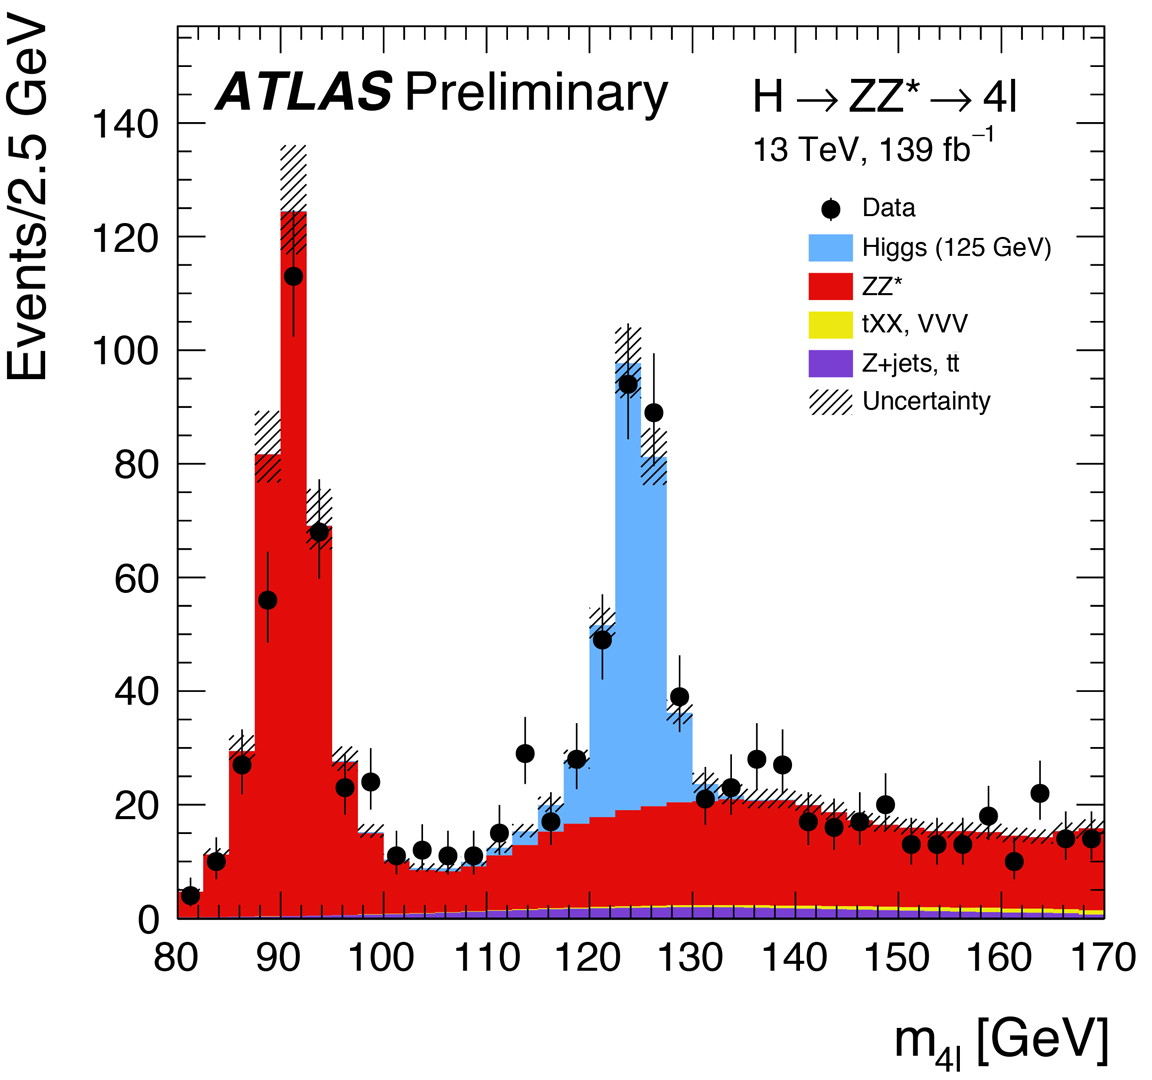
\includegraphics[width=0.6\linewidth]{./res/gfx/higgs.jpg}
  \caption{Invariant 4-lepton invariant mass of reconstructed events in the ATLAS detector for $H \rightarrow ZZ* \rightarrow 4\ell$ process, the famous plot signifying the presence of the Higgs boson.}
  \label{fig:higgs}
\end{figure}

An example of one such plot is given in Fig.~\ref{fig:higgs}. A simulation (rather, a ridiculously large number of them) was carried out that modeled the creation of a Higgs boson, its decay into a two $Z$ bosons, and their decay into four charged leptons, and the resultant distributions of the center of mass of the four leptons were recorded and plotted. The normal production of the two $Z$ bosons is shown in red (i.e. without a Higgs boson), and the process involving the Higgs is shown in blue. This comparison between the \textit{signal}, the process in question, and the \textit{background}, the expected results from the process without the new particle, is what illuminates new particles. The mass at the blue peak in this plot is equal to the mass of the Higgs boson, and the statistical uncertaintly is good enough to conclude, beyond a shadow of a doubt, that this particle exists. This particular plot came from more recent studies into ``cleaner'' Higgs production processes, but a similar-looking distribution was found back in 2012, and similar, real detector data was produced shortly afterwards that confirmed the existance of the Higgs boson. See Ref.~\cite{Aad_2020} for more information.

Evidently, it is extremely helpful to have a theoretical framework that is able to match what is seen in the detectors so that we can make predictions with that framework. This calls for the usage of complex simulation programs that model the entire chain of events starting from the ``hard scattering'' process, which is the initial collision of the protons, all the way to simulating the detector structure and how it behaves when the particles from the collision fly through it. We then read the output that the simulated detector shows us, and we can analyze the exact same things as done in experiment to make very accurate comparisons and predictions.

The reason that this must be \textit{simulated}, rather than just plugged into a calculator or some mathematical subroutine, is due to the myriad considerations that must be taken into account when talking about particle interactions at such a small scale. There are a number of different forces at play, namely the strong nuclear force, the weak nuclear force, and the electromagnetic force. Additionally, the sheer number of particles present in the system at any given time is large enough that our analytical equations simply cannot be solved by any known method without taking insanely crude approximations, which would ruin the main goal of acquiring physically sensible results.


\subsection{Physics Challenges}\label{sec:Sim-Considerations}

As one would expect, though, simulating these processes is still a huge challenge. As mentioned before, it is not simply a matter of momentum/energy conservation and other simple properties; there are a multitude of quantum mechanical phenomena that occur on this energy scale, the most notable of which come from Quantum Chromodynamics (QCD), or the strong force. Essentially, the constituents of protons, which are called \textit{quarks}, experience a force similar to that of normal electromagnetism, but opposite in some respects. For instance, bringing two electrons closer together increases the repulsion between them, since like charges repel. Similarly, bringing a proton and an electron closer together will increase the attraction between the two. Quarks, on the other hand, have the opposite property, where the closer you bring them together the less they feel like doing anything at all, and the further you bring them apart, the stronger the force between them becomes. This force is so strong that they actually cannot exist on their own: if you try and break two of them apart, at some point the energy required will be so high that two entirely new quarks will spontaneously form and bind with the two existing quarks and create new states called \textit{hadrons}, of which protons and neutrons are examples. This is manifested mathematically in that the strong/QCD coupling, $\alpha_s$, when evaluated at larger energy scales is smaller than when it is evaluated at smaller energy scales.

The reason this is an important consideration is that such a property admits significantly more complicated behavior during a collision. The protons are brought to such a high energy that, upon colliding and splitting particles out in all directions, the strong coupling is sufficiently small to consider the quarks as ``free'', meaning they don't form hadrons. In this respect, they are essentially just a bunch of electrons. However, after some more time passes, the changing distance/energy scales begin to increase the value of the coupling. At this stage, the quarks are no longer free, and they begin to hadronize. The behavior of interacting hadrons is no longer anywhere near as simple as the interacting free particles, since the substructure of the hadrons must be taken into account. 

Further, before hadronization occurs, the free quarks will radiate gluons, particles that are similar to photons but also feel the strong force like the quarks. Often, due to the energetic nature of the collision, there will be a large number of emitted gluons with high energy, that then may decay into quark/anti-quark pairs, which may then subsequently radiate further. Due to this, there are often a very large quantity of quarks/anti-quarks present once hadronization begins, further exacerbating the problem.

To avoid being too pessimistic, I will make one final note about what makes this so difficult. Currently, our frameworks in theoretical physics admit solutions that are represented by an infinite series of terms, called \textit{perturbation theory}. Essentially, this involves writing a function as an expansion in some small parameter $\lambda$ like so:

\begin{equation}
  f(x) = a_0 + \lambda a_1(x) + \lambda^2 a_2(x) + \lambda^3 a_3(x) + \ldots.\label{eq:1-intro-perturbation}
\end{equation}

Usually, $\lambda$ is the coupling for particles involved in a particular reaction. For a single interaction, there is only one factor, but as you consider more interactions, more factors of the coupling will be included. For instance, considering a quark emitting one single gluon, there is only 1 interaction, that being the interaction between the quark and the gluon. However, if we consider a chain of quark radiation, there are multiple decays and interactions between the quarks and the gluons. Any part of given process technically has a non-zero probability of occurring, meaning the full infinite series is the ``full,'' ``correct'' answer. Fortunately, the ``small parameter'' is usually sufficiently small such that we can only consider the first few terms and have the result be moderately accurate. In other words, considering only the single interaction is usually a good enough estimation for the entire process containing the infinite number of interactions.

\subsection{Project Goals}

The previous section was very general, encompassing the general idea of what should be considered to model such processes (and make calculations in general). Of course, I cannot include everything in my project, so I will make a few additional considerations.

First, for a simulation such as this, I will start by including only interactions that are represented by the first term in the aforementioned perturbative series. For instance, instead of a quark radiating a gluon which then splits into a quark/anti-quark pair and so on, I will consider only the radiation of a single gluon at a time. By virtue of perturbation theory, this will already be a decent approximation itself, at least in the high energy regime where the coupling actually remains small.

Second, modeling the entire process start to finish, i.e. from hard scattering to simulating the detector, would be an absolutely monstrous task. Most if not every program out there for simulating these processes only focuses on a subset of the full run. For instance, \textsc{MadGraph5} largely focuses on the hard scattering process, i.e. generating events that occur immediately after the collision and before any quark radiation. \textsc{Pythia8} and \textsc{Herwig++} can do this too, as well as taking into account the parton showering elements. \textsc{Geant4} focuses only on the detector simulation, and takes as input the output of \textsc{Pythia8}, \textsc{Herwig7}, or any other parton showering program. My project will focus primarily on the hard scattering process as well as the parton showering, before hadronization. I will not attempt to simulate the detector structure.

Unfortunately, due to the nature of the process I chose to simulate, namely $pp \rightarrow Z/\gamma^* \rightarrow \mu^+\mu^-$, which corresponds to the two protons interacting, exchanging a $Z$-boson or photon, then emitting two muons, is incompatible with the leading order parton showering algorithm, specifically with regards to using the outputs from the former for the latter. In principle, if I was considering higher orders, I could generate events with the muons then shower them by having them emit \textit{photons}, but the leading order (and simplest) method for implementing parton showering is by \textit{quarks} radiating \textit{gluons}. Therefore, the hard scattering and parton showering parts will simply be separate, but they will still be valid in their own regimes.



%%% Local Variables:
%%% mode: LaTeX
%%% TeX-master: "../../FinalMilestone"
%%% End:
